% Options for packages loaded elsewhere
\PassOptionsToPackage{unicode}{hyperref}
\PassOptionsToPackage{hyphens}{url}
%
\documentclass[
]{article}
\usepackage{amsmath,amssymb}
\usepackage{iftex}
\ifPDFTeX
  \usepackage[T1]{fontenc}
  \usepackage[utf8]{inputenc}
  \usepackage{textcomp} % provide euro and other symbols
\else % if luatex or xetex
  \usepackage{unicode-math} % this also loads fontspec
  \defaultfontfeatures{Scale=MatchLowercase}
  \defaultfontfeatures[\rmfamily]{Ligatures=TeX,Scale=1}
\fi
\usepackage{lmodern}
\ifPDFTeX\else
  % xetex/luatex font selection
\fi
% Use upquote if available, for straight quotes in verbatim environments
\IfFileExists{upquote.sty}{\usepackage{upquote}}{}
\IfFileExists{microtype.sty}{% use microtype if available
  \usepackage[]{microtype}
  \UseMicrotypeSet[protrusion]{basicmath} % disable protrusion for tt fonts
}{}
\makeatletter
\@ifundefined{KOMAClassName}{% if non-KOMA class
  \IfFileExists{parskip.sty}{%
    \usepackage{parskip}
  }{% else
    \setlength{\parindent}{0pt}
    \setlength{\parskip}{6pt plus 2pt minus 1pt}}
}{% if KOMA class
  \KOMAoptions{parskip=half}}
\makeatother
\usepackage{xcolor}
\usepackage[margin=1in]{geometry}
\usepackage{color}
\usepackage{fancyvrb}
\newcommand{\VerbBar}{|}
\newcommand{\VERB}{\Verb[commandchars=\\\{\}]}
\DefineVerbatimEnvironment{Highlighting}{Verbatim}{commandchars=\\\{\}}
% Add ',fontsize=\small' for more characters per line
\usepackage{framed}
\definecolor{shadecolor}{RGB}{248,248,248}
\newenvironment{Shaded}{\begin{snugshade}}{\end{snugshade}}
\newcommand{\AlertTok}[1]{\textcolor[rgb]{0.94,0.16,0.16}{#1}}
\newcommand{\AnnotationTok}[1]{\textcolor[rgb]{0.56,0.35,0.01}{\textbf{\textit{#1}}}}
\newcommand{\AttributeTok}[1]{\textcolor[rgb]{0.13,0.29,0.53}{#1}}
\newcommand{\BaseNTok}[1]{\textcolor[rgb]{0.00,0.00,0.81}{#1}}
\newcommand{\BuiltInTok}[1]{#1}
\newcommand{\CharTok}[1]{\textcolor[rgb]{0.31,0.60,0.02}{#1}}
\newcommand{\CommentTok}[1]{\textcolor[rgb]{0.56,0.35,0.01}{\textit{#1}}}
\newcommand{\CommentVarTok}[1]{\textcolor[rgb]{0.56,0.35,0.01}{\textbf{\textit{#1}}}}
\newcommand{\ConstantTok}[1]{\textcolor[rgb]{0.56,0.35,0.01}{#1}}
\newcommand{\ControlFlowTok}[1]{\textcolor[rgb]{0.13,0.29,0.53}{\textbf{#1}}}
\newcommand{\DataTypeTok}[1]{\textcolor[rgb]{0.13,0.29,0.53}{#1}}
\newcommand{\DecValTok}[1]{\textcolor[rgb]{0.00,0.00,0.81}{#1}}
\newcommand{\DocumentationTok}[1]{\textcolor[rgb]{0.56,0.35,0.01}{\textbf{\textit{#1}}}}
\newcommand{\ErrorTok}[1]{\textcolor[rgb]{0.64,0.00,0.00}{\textbf{#1}}}
\newcommand{\ExtensionTok}[1]{#1}
\newcommand{\FloatTok}[1]{\textcolor[rgb]{0.00,0.00,0.81}{#1}}
\newcommand{\FunctionTok}[1]{\textcolor[rgb]{0.13,0.29,0.53}{\textbf{#1}}}
\newcommand{\ImportTok}[1]{#1}
\newcommand{\InformationTok}[1]{\textcolor[rgb]{0.56,0.35,0.01}{\textbf{\textit{#1}}}}
\newcommand{\KeywordTok}[1]{\textcolor[rgb]{0.13,0.29,0.53}{\textbf{#1}}}
\newcommand{\NormalTok}[1]{#1}
\newcommand{\OperatorTok}[1]{\textcolor[rgb]{0.81,0.36,0.00}{\textbf{#1}}}
\newcommand{\OtherTok}[1]{\textcolor[rgb]{0.56,0.35,0.01}{#1}}
\newcommand{\PreprocessorTok}[1]{\textcolor[rgb]{0.56,0.35,0.01}{\textit{#1}}}
\newcommand{\RegionMarkerTok}[1]{#1}
\newcommand{\SpecialCharTok}[1]{\textcolor[rgb]{0.81,0.36,0.00}{\textbf{#1}}}
\newcommand{\SpecialStringTok}[1]{\textcolor[rgb]{0.31,0.60,0.02}{#1}}
\newcommand{\StringTok}[1]{\textcolor[rgb]{0.31,0.60,0.02}{#1}}
\newcommand{\VariableTok}[1]{\textcolor[rgb]{0.00,0.00,0.00}{#1}}
\newcommand{\VerbatimStringTok}[1]{\textcolor[rgb]{0.31,0.60,0.02}{#1}}
\newcommand{\WarningTok}[1]{\textcolor[rgb]{0.56,0.35,0.01}{\textbf{\textit{#1}}}}
\usepackage{graphicx}
\makeatletter
\def\maxwidth{\ifdim\Gin@nat@width>\linewidth\linewidth\else\Gin@nat@width\fi}
\def\maxheight{\ifdim\Gin@nat@height>\textheight\textheight\else\Gin@nat@height\fi}
\makeatother
% Scale images if necessary, so that they will not overflow the page
% margins by default, and it is still possible to overwrite the defaults
% using explicit options in \includegraphics[width, height, ...]{}
\setkeys{Gin}{width=\maxwidth,height=\maxheight,keepaspectratio}
% Set default figure placement to htbp
\makeatletter
\def\fps@figure{htbp}
\makeatother
\setlength{\emergencystretch}{3em} % prevent overfull lines
\providecommand{\tightlist}{%
  \setlength{\itemsep}{0pt}\setlength{\parskip}{0pt}}
\setcounter{secnumdepth}{-\maxdimen} % remove section numbering
\ifLuaTeX
  \usepackage{selnolig}  % disable illegal ligatures
\fi
\IfFileExists{bookmark.sty}{\usepackage{bookmark}}{\usepackage{hyperref}}
\IfFileExists{xurl.sty}{\usepackage{xurl}}{} % add URL line breaks if available
\urlstyle{same}
\hypersetup{
  pdftitle={Week 10 Challenge},
  pdfauthor={Ariel Quek},
  hidelinks,
  pdfcreator={LaTeX via pandoc}}

\title{Week 10 Challenge}
\author{Ariel Quek}
\date{2023-10-30}

\begin{document}
\maketitle

\begin{Shaded}
\begin{Highlighting}[]
\NormalTok{knitr}\SpecialCharTok{::}\NormalTok{opts\_chunk}\SpecialCharTok{$}\FunctionTok{set}\NormalTok{(}\AttributeTok{echo =} \ConstantTok{TRUE}\NormalTok{)}
\end{Highlighting}
\end{Shaded}

\hypertarget{week-10-challenge}{%
\subsection{Week 10 Challenge}\label{week-10-challenge}}

\hypertarget{step-1}{%
\subsubsection{Step 1}\label{step-1}}

\emph{Downloading data set (API)}

\begin{Shaded}
\begin{Highlighting}[]
\FunctionTok{library}\NormalTok{(httr)}
\end{Highlighting}
\end{Shaded}

\begin{verbatim}
## Warning: package 'httr' was built under R version 4.2.3
\end{verbatim}

\begin{Shaded}
\begin{Highlighting}[]
\FunctionTok{library}\NormalTok{(jsonlite)}
\end{Highlighting}
\end{Shaded}

\begin{verbatim}
## Warning: package 'jsonlite' was built under R version 4.2.3
\end{verbatim}

\begin{Shaded}
\begin{Highlighting}[]
\FunctionTok{library}\NormalTok{(tidyverse)}
\end{Highlighting}
\end{Shaded}

\begin{verbatim}
## Warning: package 'tidyverse' was built under R version 4.2.3
\end{verbatim}

\begin{verbatim}
## Warning: package 'ggplot2' was built under R version 4.2.3
\end{verbatim}

\begin{verbatim}
## Warning: package 'tibble' was built under R version 4.2.1
\end{verbatim}

\begin{verbatim}
## Warning: package 'tidyr' was built under R version 4.2.2
\end{verbatim}

\begin{verbatim}
## Warning: package 'readr' was built under R version 4.2.3
\end{verbatim}

\begin{verbatim}
## Warning: package 'purrr' was built under R version 4.2.2
\end{verbatim}

\begin{verbatim}
## Warning: package 'dplyr' was built under R version 4.2.2
\end{verbatim}

\begin{verbatim}
## Warning: package 'stringr' was built under R version 4.2.2
\end{verbatim}

\begin{verbatim}
## Warning: package 'forcats' was built under R version 4.2.3
\end{verbatim}

\begin{verbatim}
## Warning: package 'lubridate' was built under R version 4.2.3
\end{verbatim}

\begin{verbatim}
## -- Attaching core tidyverse packages ------------------------ tidyverse 2.0.0 --
## v dplyr     1.1.0     v readr     2.1.4
## v forcats   1.0.0     v stringr   1.5.0
## v ggplot2   3.4.3     v tibble    3.1.8
## v lubridate 1.9.2     v tidyr     1.3.0
## v purrr     1.0.1     
## -- Conflicts ------------------------------------------ tidyverse_conflicts() --
## x dplyr::filter()  masks stats::filter()
## x purrr::flatten() masks jsonlite::flatten()
## x dplyr::lag()     masks stats::lag()
## i Use the ]8;;http://conflicted.r-lib.org/conflicted package]8;; to force all conflicts to become errors
\end{verbatim}

\emph{Retrieving data}

\begin{Shaded}
\begin{Highlighting}[]
\NormalTok{historic\_state\_data\_url }\OtherTok{\textless{}{-}} \StringTok{"https://api.covidactnow.org/v2/states.timeseries.json?apiKey=aee461090f09499f86335e3630089532"}

\NormalTok{raw\_data }\OtherTok{\textless{}{-}} \FunctionTok{GET}\NormalTok{(historic\_state\_data\_url)}
\end{Highlighting}
\end{Shaded}

\hypertarget{step-2}{%
\subsubsection{Step 2}\label{step-2}}

\emph{Converting data to a dataframe}

\begin{Shaded}
\begin{Highlighting}[]
\NormalTok{data }\OtherTok{\textless{}{-}} \FunctionTok{fromJSON}\NormalTok{(}\FunctionTok{rawToChar}\NormalTok{(raw\_data}\SpecialCharTok{$}\NormalTok{content))}
\end{Highlighting}
\end{Shaded}

\hypertarget{step-3}{%
\subsubsection{Step 3}\label{step-3}}

\emph{Get a glimpse of data-set}

\begin{Shaded}
\begin{Highlighting}[]
\FunctionTok{glimpse}\NormalTok{(data)}
\end{Highlighting}
\end{Shaded}

\begin{verbatim}
## Rows: 53
## Columns: 25
## $ fips                           <chr> "02", "01", "05", "04", "06", "08", "09~
## $ country                        <chr> "US", "US", "US", "US", "US", "US", "US~
## $ state                          <chr> "AK", "AL", "AR", "AZ", "CA", "CO", "CT~
## $ county                         <lgl> NA, NA, NA, NA, NA, NA, NA, NA, NA, NA,~
## $ hsa                            <lgl> NA, NA, NA, NA, NA, NA, NA, NA, NA, NA,~
## $ hsaName                        <lgl> NA, NA, NA, NA, NA, NA, NA, NA, NA, NA,~
## $ level                          <chr> "state", "state", "state", "state", "st~
## $ lat                            <lgl> NA, NA, NA, NA, NA, NA, NA, NA, NA, NA,~
## $ locationId                     <chr> "iso1:us#iso2:us-ak", "iso1:us#iso2:us-~
## $ long                           <lgl> NA, NA, NA, NA, NA, NA, NA, NA, NA, NA,~
## $ population                     <int> 731545, 4903185, 3017804, 7278717, 3951~
## $ hsaPopulation                  <int> NA, NA, NA, NA, NA, NA, NA, NA, NA, NA,~
## $ metrics                        <df[,14]> <data.frame[26 x 14]>
## $ riskLevels                     <df[,6]> <data.frame[26 x 6]>
## $ cdcTransmissionLevel           <int> 2, 4, 3, 3, 1, 4, 4, 1, 4, 4, 2, 3,~
## $ communityLevels                <df[,2]> <data.frame[26 x 2]>
## $ actuals                        <df[,19]> <data.frame[26 x 19]>
## $ annotations                    <df[,30]> <data.frame[26 x 30]>
## $ lastUpdatedDate                <chr> "2023-10-30", "2023-10-30", "2023-10~
## $ url                            <chr> "https://covidactnow.org/us/alaska-ak",~
## $ metricsTimeseries              <list> [<data.frame[1334 x 14]>], [<data.fr~
## $ actualsTimeseries              <list> [<data.frame[1334 x 20]>], [<data.f~
## $ riskLevelsTimeseries           <list> [<data.frame[1334 x 3]>], [<data.fr~
## $ cdcTransmissionLevelTimeseries <list> [<data.frame[1334 x 2]>], [<data.frame[~
## $ communityLevelsTimeseries      <list> [<data.frame[1334 x 3]>], [<data.frame[~
\end{verbatim}

\hypertarget{step-4}{%
\subsubsection{Step 4}\label{step-4}}

We will work on the following questions:

\begin{enumerate}
\def\labelenumi{\roman{enumi}.}
\item
  What is the population in various states of U.S.A?
\item
  What fraction of the population was infected ?
\item
  What fraction of infected persons recovered ?
\item
  What fraction of the population is currently vaccinated ? \emph{the
  above do not need historical data}
\item
  What was the transmission-like in the various states ?
\item
  How did the disease progress since it started ? \emph{the above needs
  us to plot values of transmission and cases on a periodical basis --
  requires time-series values}
\end{enumerate}

\hypertarget{step-5}{%
\subsubsection{Step 5}\label{step-5}}

\emph{Extracting time-series data from the data-frame}

\begin{Shaded}
\begin{Highlighting}[]
\NormalTok{time\_series }\OtherTok{\textless{}{-}}\NormalTok{ data }\SpecialCharTok{\%\textgreater{}\%} \FunctionTok{unnest}\NormalTok{(actualsTimeseries) }
\CommentTok{\# \textless{}{-} to unravel the contents of a dataframe within a dataframe, use unnest}
\end{Highlighting}
\end{Shaded}

\emph{Creating a new dataframe with the needed data}

\begin{Shaded}
\begin{Highlighting}[]
\NormalTok{time\_series\_transmission }\OtherTok{\textless{}{-}} \FunctionTok{tibble}\NormalTok{(}\AttributeTok{Date=}\NormalTok{time\_series}\SpecialCharTok{$}\NormalTok{cdcTransmissionLevelTimeseries[[}\FunctionTok{which}\NormalTok{(data}\SpecialCharTok{$}\NormalTok{state}\SpecialCharTok{==}\StringTok{"CA"}\NormalTok{)]]}\SpecialCharTok{$}\NormalTok{date)}

\CommentTok{\# Transmission levels in each state}
\NormalTok{time\_series\_transmission}\SpecialCharTok{$}\NormalTok{Alaska }\OtherTok{\textless{}{-}}\NormalTok{ time\_series}\SpecialCharTok{$}\NormalTok{cdcTransmissionLevelTimeseries[[}\FunctionTok{which}\NormalTok{(data}\SpecialCharTok{$}\NormalTok{state}\SpecialCharTok{==}\StringTok{"AK"}\NormalTok{)]]}\SpecialCharTok{$}\NormalTok{cdcTransmissionLevel}

\NormalTok{time\_series\_transmission}\SpecialCharTok{$}\NormalTok{California }\OtherTok{\textless{}{-}}\NormalTok{ time\_series}\SpecialCharTok{$}\NormalTok{cdcTransmissionLevelTimeseries[[}\FunctionTok{which}\NormalTok{(data}\SpecialCharTok{$}\NormalTok{state}\SpecialCharTok{==}\StringTok{"CA"}\NormalTok{)]]}\SpecialCharTok{$}\NormalTok{cdcTransmissionLevel}

\NormalTok{time\_series\_transmission}\SpecialCharTok{$}\NormalTok{New\_Jersey }\OtherTok{\textless{}{-}}\NormalTok{ time\_series}\SpecialCharTok{$}\NormalTok{cdcTransmissionLevelTimeseries[[}\FunctionTok{which}\NormalTok{(data}\SpecialCharTok{$}\NormalTok{state}\SpecialCharTok{==}\StringTok{"NJ"}\NormalTok{)]]}\SpecialCharTok{$}\NormalTok{cdcTransmissionLevel}

\NormalTok{time\_series\_transmission}\SpecialCharTok{$}\NormalTok{Tennessee }\OtherTok{\textless{}{-}}\NormalTok{ time\_series}\SpecialCharTok{$}\NormalTok{cdcTransmissionLevelTimeseries[[}\FunctionTok{which}\NormalTok{(data}\SpecialCharTok{$}\NormalTok{state}\SpecialCharTok{==}\StringTok{"TN"}\NormalTok{)]]}\SpecialCharTok{$}\NormalTok{cdcTransmissionLevel}

\NormalTok{time\_series\_transmission}\SpecialCharTok{$}\NormalTok{District\_of\_Columbia }\OtherTok{\textless{}{-}}\NormalTok{ time\_series}\SpecialCharTok{$}\NormalTok{cdcTransmissionLevelTimeseries[[}\FunctionTok{which}\NormalTok{(data}\SpecialCharTok{$}\NormalTok{state}\SpecialCharTok{==}\StringTok{"DC"}\NormalTok{)]]}\SpecialCharTok{$}\NormalTok{cdcTransmissionLevel}

\FunctionTok{print}\NormalTok{(}\FunctionTok{head}\NormalTok{(time\_series\_transmission))}
\end{Highlighting}
\end{Shaded}

\begin{verbatim}
## # A tibble: 6 x 6
##   Date       Alaska California New_Jersey Tennessee District_of_Columbia
##   <chr>       <int>      <int>      <int>     <int>                <int>
## 1 2020-03-01      0          0          0         0                    0
## 2 2020-03-02      0          0          0         0                    0
## 3 2020-03-03      0          0          0         0                    0
## 4 2020-03-04      0          0          0         0                    0
## 5 2020-03-05      0          0          0         0                    0
## 6 2020-03-06      0          0          0         0                    0
\end{verbatim}

\emph{Selecting cases of each states from a new data-frame with dates}

\begin{Shaded}
\begin{Highlighting}[]
\CommentTok{\# New data{-}frame with dates}
\NormalTok{time\_series\_cases }\OtherTok{\textless{}{-}} \FunctionTok{list}\NormalTok{(}\AttributeTok{Alaska =}\NormalTok{ time\_series }\SpecialCharTok{\%\textgreater{}\%} \FunctionTok{filter}\NormalTok{(state}\SpecialCharTok{==}\StringTok{"AK"}\NormalTok{) }\SpecialCharTok{\%\textgreater{}\%} \FunctionTok{select}\NormalTok{(date,cases))}
\CommentTok{\# Cases of each state}
\NormalTok{time\_series\_cases}\SpecialCharTok{$}\NormalTok{California }\OtherTok{\textless{}{-}}\NormalTok{ time\_series }\SpecialCharTok{\%\textgreater{}\%} \FunctionTok{filter}\NormalTok{(state}\SpecialCharTok{==}\StringTok{"CA"}\NormalTok{) }\SpecialCharTok{\%\textgreater{}\%} \FunctionTok{select}\NormalTok{(date,cases)}
\NormalTok{time\_series\_cases}\SpecialCharTok{$}\NormalTok{New\_Jersey }\OtherTok{\textless{}{-}}\NormalTok{ time\_series }\SpecialCharTok{\%\textgreater{}\%} \FunctionTok{filter}\NormalTok{(state}\SpecialCharTok{==}\StringTok{"NJ"}\NormalTok{) }\SpecialCharTok{\%\textgreater{}\%} \FunctionTok{select}\NormalTok{(date,cases)}
\NormalTok{time\_series\_cases}\SpecialCharTok{$}\NormalTok{Tennessee }\OtherTok{\textless{}{-}}\NormalTok{ time\_series }\SpecialCharTok{\%\textgreater{}\%} \FunctionTok{filter}\NormalTok{(state}\SpecialCharTok{==}\StringTok{"TN"}\NormalTok{) }\SpecialCharTok{\%\textgreater{}\%} \FunctionTok{select}\NormalTok{(date,cases)}
\NormalTok{time\_series\_cases}\SpecialCharTok{$}\NormalTok{District\_of\_Columbia }\OtherTok{\textless{}{-}}\NormalTok{ time\_series }\SpecialCharTok{\%\textgreater{}\%} \FunctionTok{filter}\NormalTok{(state}\SpecialCharTok{==}\StringTok{"DC"}\NormalTok{) }\SpecialCharTok{\%\textgreater{}\%} \FunctionTok{select}\NormalTok{(date,cases)}
\end{Highlighting}
\end{Shaded}

\hypertarget{step-6}{%
\subsubsection{Step 6}\label{step-6}}

Visualising the data

\begin{Shaded}
\begin{Highlighting}[]
\FunctionTok{ggplot}\NormalTok{(data, }\FunctionTok{aes}\NormalTok{(}\AttributeTok{x=}\NormalTok{state,}\AttributeTok{y=}\NormalTok{population)) }\SpecialCharTok{+} \FunctionTok{geom\_bar}\NormalTok{(}\AttributeTok{stat=}\StringTok{"identity"}\NormalTok{) }\SpecialCharTok{+}\FunctionTok{labs}\NormalTok{(}\AttributeTok{x=}\StringTok{"States"}\NormalTok{,}\AttributeTok{y=}\StringTok{"Population"}\NormalTok{) }\SpecialCharTok{+} \FunctionTok{theme\_bw}\NormalTok{()}
\end{Highlighting}
\end{Shaded}

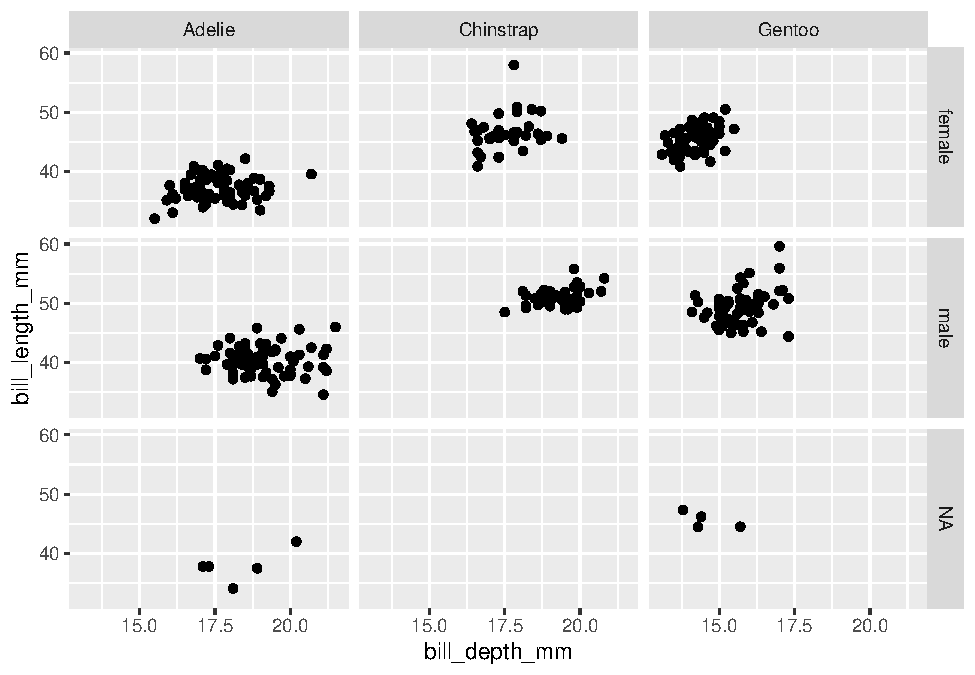
\includegraphics{Week-11-Challenge_files/figure-latex/unnamed-chunk-8-1.pdf}

\begin{Shaded}
\begin{Highlighting}[]
\FunctionTok{ggplot}\NormalTok{(data, }\FunctionTok{aes}\NormalTok{(}\AttributeTok{x=}\NormalTok{state,}\AttributeTok{y=}\NormalTok{(data}\SpecialCharTok{$}\NormalTok{actuals}\SpecialCharTok{$}\NormalTok{cases}\SpecialCharTok{/}\NormalTok{population))) }\SpecialCharTok{+} \FunctionTok{geom\_bar}\NormalTok{(}\AttributeTok{stat=}\StringTok{"identity"}\NormalTok{) }\SpecialCharTok{+} \FunctionTok{labs}\NormalTok{(}\AttributeTok{x=}\StringTok{"States"}\NormalTok{,}\AttributeTok{y=}\StringTok{"Infected (\%)"}\NormalTok{)}\SpecialCharTok{+}\FunctionTok{theme\_bw}\NormalTok{()}
\end{Highlighting}
\end{Shaded}

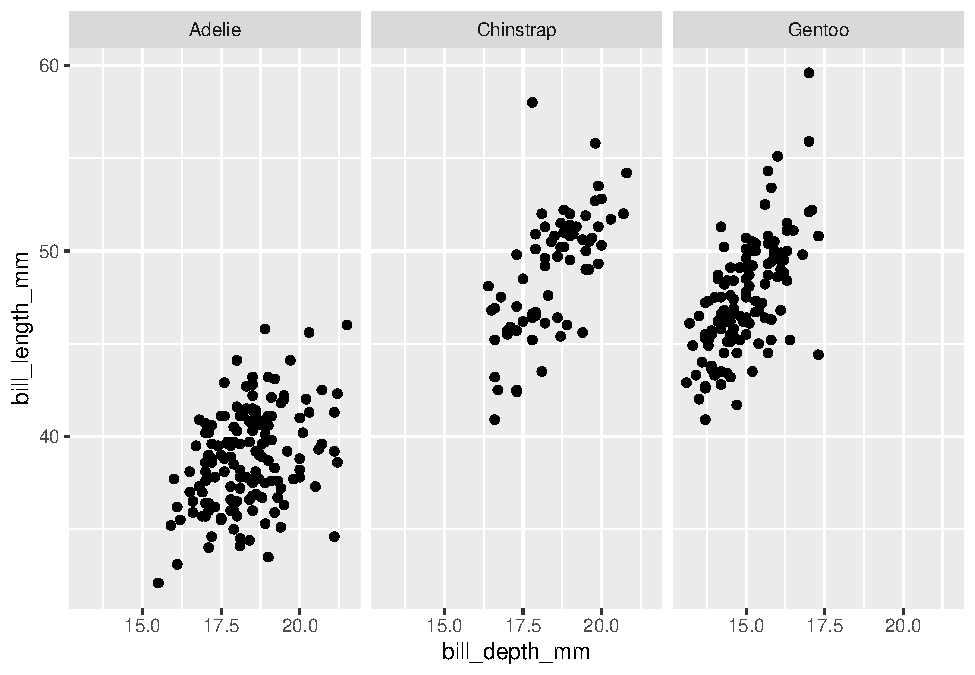
\includegraphics{Week-11-Challenge_files/figure-latex/unnamed-chunk-9-1.pdf}

\begin{Shaded}
\begin{Highlighting}[]
\NormalTok{time\_series\_transmission[}\FunctionTok{seq}\NormalTok{(}\DecValTok{1}\NormalTok{,}\DecValTok{1300}\NormalTok{,}\AttributeTok{by=}\DecValTok{100}\NormalTok{),]}\SpecialCharTok{\%\textgreater{}\%}
  \FunctionTok{pivot\_longer}\NormalTok{(}\AttributeTok{cols=}\NormalTok{Alaska}\SpecialCharTok{:}\NormalTok{District\_of\_Columbia,}\AttributeTok{names\_to=}\StringTok{"Countries"}\NormalTok{,}\AttributeTok{values\_to=}\StringTok{"Transmission"}\NormalTok{) }\SpecialCharTok{\%\textgreater{}\%}
  \FunctionTok{ggplot}\NormalTok{(}\FunctionTok{aes}\NormalTok{(}\AttributeTok{x=}\NormalTok{Date,}\AttributeTok{y=}\NormalTok{Transmission,}\AttributeTok{colour=}\NormalTok{Countries,}\AttributeTok{group=}\NormalTok{Countries)) }\SpecialCharTok{+} 
  \FunctionTok{geom\_point}\NormalTok{(}\AttributeTok{show.legend=}\ConstantTok{TRUE}\NormalTok{) }\SpecialCharTok{+} 
  \FunctionTok{labs}\NormalTok{(}\AttributeTok{x=}\StringTok{"Date"}\NormalTok{,}\AttributeTok{y=}\StringTok{"Transmission Level"}\NormalTok{) }\SpecialCharTok{+}
  \FunctionTok{theme\_bw}\NormalTok{()}
\end{Highlighting}
\end{Shaded}

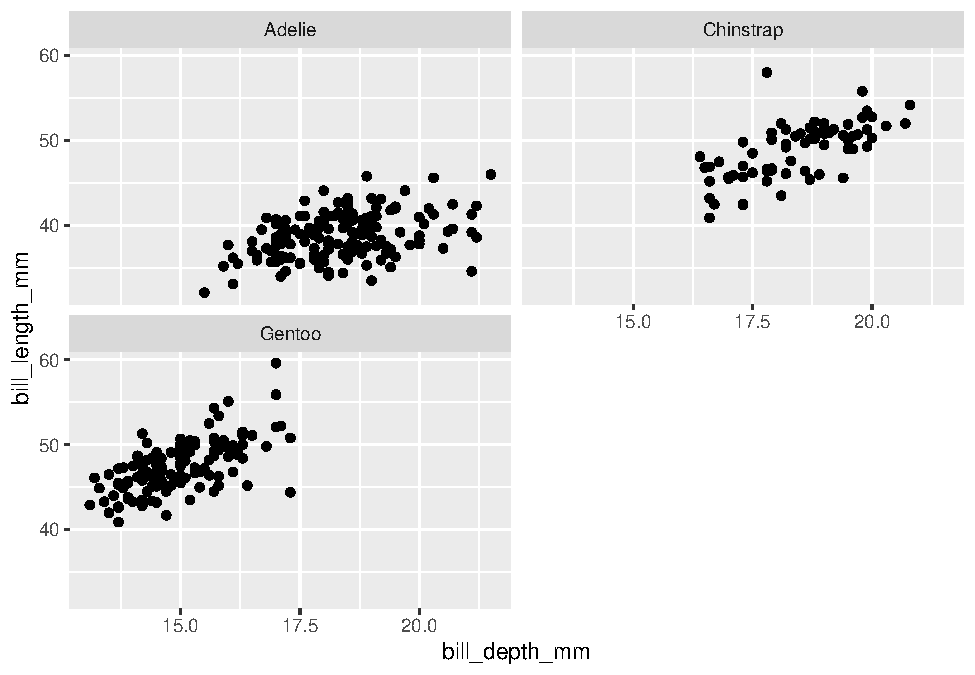
\includegraphics{Week-11-Challenge_files/figure-latex/unnamed-chunk-10-1.pdf}
Representing the data

\begin{Shaded}
\begin{Highlighting}[]
\NormalTok{data\_to\_plot }\OtherTok{\textless{}{-}} \FunctionTok{tibble}\NormalTok{(}\AttributeTok{Date\_Alaska =}\NormalTok{ time\_series\_cases}\SpecialCharTok{$}\NormalTok{Alaska}\SpecialCharTok{$}\NormalTok{date[}\FunctionTok{seq}\NormalTok{(}\DecValTok{1}\NormalTok{,}\DecValTok{1300}\NormalTok{,}\AttributeTok{by=}\DecValTok{100}\NormalTok{)],}
                       \AttributeTok{Cases\_Alaska =}\NormalTok{ time\_series\_cases}\SpecialCharTok{$}\NormalTok{Alaska}\SpecialCharTok{$}\NormalTok{cases[}\FunctionTok{seq}\NormalTok{(}\DecValTok{1}\NormalTok{,}\DecValTok{1300}\NormalTok{,}\AttributeTok{by=}\DecValTok{100}\NormalTok{)], }
                       \AttributeTok{Date\_California =}\NormalTok{ time\_series\_cases}\SpecialCharTok{$}\NormalTok{California}\SpecialCharTok{$}\NormalTok{date[}\FunctionTok{seq}\NormalTok{(}\DecValTok{1}\NormalTok{,}\DecValTok{1300}\NormalTok{,}\AttributeTok{by=}\DecValTok{100}\NormalTok{)],}
                       \AttributeTok{Cases\_California =}\NormalTok{ time\_series\_cases}\SpecialCharTok{$}\NormalTok{California}\SpecialCharTok{$}\NormalTok{cases[}\FunctionTok{seq}\NormalTok{(}\DecValTok{1}\NormalTok{,}\DecValTok{1300}\NormalTok{,}\AttributeTok{by=}\DecValTok{100}\NormalTok{)],}
                       \AttributeTok{Date\_New\_Jersey =}\NormalTok{ time\_series\_cases}\SpecialCharTok{$}\NormalTok{New\_Jersey}\SpecialCharTok{$}\NormalTok{date[}\FunctionTok{seq}\NormalTok{(}\DecValTok{1}\NormalTok{,}\DecValTok{1300}\NormalTok{,}\AttributeTok{by=}\DecValTok{100}\NormalTok{)],}
                       \AttributeTok{Cases\_New\_Jersey =}\NormalTok{ time\_series\_cases}\SpecialCharTok{$}\NormalTok{New\_Jersey}\SpecialCharTok{$}\NormalTok{cases[}\FunctionTok{seq}\NormalTok{(}\DecValTok{1}\NormalTok{,}\DecValTok{1300}\NormalTok{,}\AttributeTok{by=}\DecValTok{100}\NormalTok{)],}
                       \AttributeTok{Date\_Tennessee =}\NormalTok{ time\_series\_cases}\SpecialCharTok{$}\NormalTok{Tennessee}\SpecialCharTok{$}\NormalTok{date[}\FunctionTok{seq}\NormalTok{(}\DecValTok{1}\NormalTok{,}\DecValTok{1300}\NormalTok{,}\AttributeTok{by=}\DecValTok{100}\NormalTok{)],}
                       \AttributeTok{Cases\_Tennessee =}\NormalTok{ time\_series\_cases}\SpecialCharTok{$}\NormalTok{Tennessee}\SpecialCharTok{$}\NormalTok{cases[}\FunctionTok{seq}\NormalTok{(}\DecValTok{1}\NormalTok{,}\DecValTok{1300}\NormalTok{,}\AttributeTok{by=}\DecValTok{100}\NormalTok{)],}
                       \AttributeTok{Date\_District\_of\_Columbia =}\NormalTok{ time\_series\_cases}\SpecialCharTok{$}\NormalTok{District\_of\_Columbia}\SpecialCharTok{$}\NormalTok{date[}\FunctionTok{seq}\NormalTok{(}\DecValTok{1}\NormalTok{,}\DecValTok{1300}\NormalTok{,}\AttributeTok{by=}\DecValTok{100}\NormalTok{)],}
                       \AttributeTok{Cases\_District\_of\_Columbia =}\NormalTok{ time\_series\_cases}\SpecialCharTok{$}\NormalTok{District\_of\_Columbia}\SpecialCharTok{$}\NormalTok{cases[}\FunctionTok{seq}\NormalTok{(}\DecValTok{1}\NormalTok{,}\DecValTok{1300}\NormalTok{,}\AttributeTok{by=}\DecValTok{100}\NormalTok{)])}

\NormalTok{data\_to\_plot}
\end{Highlighting}
\end{Shaded}

\begin{verbatim}
## # A tibble: 13 x 10
##    Date_Alaska Cases_Alaska Date_California Cases_California Date_New_Jersey
##    <chr>              <int> <chr>                      <int> <chr>          
##  1 2020-03-01            NA 2020-01-25                     1 2020-03-01     
##  2 2020-06-09           620 2020-05-04                 56333 2020-06-09     
##  3 2020-09-17          7413 2020-08-12                595097 2020-09-17     
##  4 2020-12-26         45247 2020-11-20               1096427 2020-12-26     
##  5 2021-04-05         63486 2021-02-28               3569578 2021-04-05     
##  6 2021-07-14         71539 2021-06-08               3798225 2021-07-14     
##  7 2021-10-22        132393 2021-09-16               4629146 2021-10-22     
##  8 2022-01-30        211117 2021-12-25               5291605 2022-01-30     
##  9 2022-05-10        252847 2022-04-04               9110544 2022-05-10     
## 10 2022-08-18        289203 2022-07-13              10365785 2022-08-18     
## 11 2022-11-26        299841 2022-10-21              11338846 2022-11-26     
## 12 2023-03-06        307377 2023-01-29              11980312 2023-03-06     
## 13 2023-06-14            NA 2023-05-09              12242634 2023-06-14     
## # i 5 more variables: Cases_New_Jersey <int>, Date_Tennessee <chr>,
## #   Cases_Tennessee <int>, Date_District_of_Columbia <chr>,
## #   Cases_District_of_Columbia <int>
\end{verbatim}

Ploting subplots

\begin{Shaded}
\begin{Highlighting}[]
\FunctionTok{install.packages}\NormalTok{(}\StringTok{"cowplot"}\NormalTok{, }\AttributeTok{repos =} \StringTok{"http://cran.us.r{-}project.org"}\NormalTok{)}
\end{Highlighting}
\end{Shaded}

\begin{verbatim}
## Installing package into 'C:/Users/Ariel/AppData/Local/R/win-library/4.2'
## (as 'lib' is unspecified)
\end{verbatim}

\begin{verbatim}
## package 'cowplot' successfully unpacked and MD5 sums checked
## 
## The downloaded binary packages are in
##  C:\Users\Ariel\AppData\Local\Temp\RtmpkVt0To\downloaded_packages
\end{verbatim}

\begin{Shaded}
\begin{Highlighting}[]
\FunctionTok{library}\NormalTok{(cowplot)}
\end{Highlighting}
\end{Shaded}

\begin{verbatim}
## Warning: package 'cowplot' was built under R version 4.2.3
\end{verbatim}

\begin{verbatim}
## 
## Attaching package: 'cowplot'
\end{verbatim}

\begin{verbatim}
## The following object is masked from 'package:lubridate':
## 
##     stamp
\end{verbatim}

\begin{Shaded}
\begin{Highlighting}[]
\NormalTok{fig1}\OtherTok{\textless{}{-}} \FunctionTok{ggplot}\NormalTok{(data\_to\_plot, }\FunctionTok{aes}\NormalTok{(}\AttributeTok{x=}\NormalTok{Date\_Alaska,}\AttributeTok{y=}\NormalTok{Cases\_Alaska)) }\SpecialCharTok{+}
  \FunctionTok{geom\_point}\NormalTok{() }\SpecialCharTok{+} \FunctionTok{labs}\NormalTok{(}\AttributeTok{x=}\StringTok{"Date"}\NormalTok{,}\AttributeTok{y=}\StringTok{"Cases"}\NormalTok{, }\AttributeTok{title=}\StringTok{"Alaska"}\NormalTok{) }\SpecialCharTok{+} \FunctionTok{theme\_bw}\NormalTok{()}

\NormalTok{fig2}\OtherTok{\textless{}{-}} \FunctionTok{ggplot}\NormalTok{(data\_to\_plot, }\FunctionTok{aes}\NormalTok{(}\AttributeTok{x=}\NormalTok{Date\_California,}\AttributeTok{y=}\NormalTok{Cases\_California)) }\SpecialCharTok{+}
  \FunctionTok{geom\_point}\NormalTok{() }\SpecialCharTok{+} \FunctionTok{labs}\NormalTok{(}\AttributeTok{x=}\StringTok{"Date"}\NormalTok{,}\AttributeTok{y=}\StringTok{"Cases"}\NormalTok{, }\AttributeTok{title=}\StringTok{"California"}\NormalTok{) }\SpecialCharTok{+} \FunctionTok{theme\_bw}\NormalTok{()}

\NormalTok{fig3}\OtherTok{\textless{}{-}} \FunctionTok{ggplot}\NormalTok{(data\_to\_plot, }\FunctionTok{aes}\NormalTok{(}\AttributeTok{x=}\NormalTok{Date\_New\_Jersey,}\AttributeTok{y=}\NormalTok{Cases\_New\_Jersey)) }\SpecialCharTok{+}
  \FunctionTok{geom\_point}\NormalTok{() }\SpecialCharTok{+} \FunctionTok{labs}\NormalTok{(}\AttributeTok{x=}\StringTok{"Date"}\NormalTok{,}\AttributeTok{y=}\StringTok{"Cases"}\NormalTok{, }\AttributeTok{title=}\StringTok{"New Jersey"}\NormalTok{) }\SpecialCharTok{+} \FunctionTok{theme\_bw}\NormalTok{()}

\NormalTok{fig4}\OtherTok{\textless{}{-}} \FunctionTok{ggplot}\NormalTok{(data\_to\_plot, }\FunctionTok{aes}\NormalTok{(}\AttributeTok{x=}\NormalTok{Date\_Tennessee,}\AttributeTok{y=}\NormalTok{Cases\_Tennessee)) }\SpecialCharTok{+}
  \FunctionTok{geom\_point}\NormalTok{() }\SpecialCharTok{+} \FunctionTok{labs}\NormalTok{(}\AttributeTok{x=}\StringTok{"Date"}\NormalTok{,}\AttributeTok{y=}\StringTok{"Cases"}\NormalTok{, }\AttributeTok{title=}\StringTok{"Tennessee"}\NormalTok{) }\SpecialCharTok{+} \FunctionTok{theme\_bw}\NormalTok{()}

\NormalTok{fig5}\OtherTok{\textless{}{-}} \FunctionTok{ggplot}\NormalTok{(data\_to\_plot, }\FunctionTok{aes}\NormalTok{(}\AttributeTok{x=}\NormalTok{Date\_District\_of\_Columbia,}\AttributeTok{y=}\NormalTok{Cases\_District\_of\_Columbia)) }\SpecialCharTok{+}
  \FunctionTok{geom\_point}\NormalTok{() }\SpecialCharTok{+} \FunctionTok{labs}\NormalTok{(}\AttributeTok{x=}\StringTok{"Date"}\NormalTok{,}\AttributeTok{y=}\StringTok{"Cases"}\NormalTok{, }\AttributeTok{title=}\StringTok{"District of Columbia"}\NormalTok{) }\SpecialCharTok{+} \FunctionTok{theme\_bw}\NormalTok{()}

\FunctionTok{plot\_grid}\NormalTok{(fig1 }\SpecialCharTok{+} \FunctionTok{theme}\NormalTok{(}\AttributeTok{legend.justification =} \FunctionTok{c}\NormalTok{(}\DecValTok{0}\NormalTok{,}\DecValTok{1}\NormalTok{)),}
\NormalTok{          fig2 }\SpecialCharTok{+} \FunctionTok{theme}\NormalTok{(}\AttributeTok{legend.justification =} \FunctionTok{c}\NormalTok{(}\DecValTok{1}\NormalTok{,}\DecValTok{0}\NormalTok{)),}
\NormalTok{          fig3 }\SpecialCharTok{+} \FunctionTok{theme}\NormalTok{(}\AttributeTok{legend.justification =} \FunctionTok{c}\NormalTok{(}\DecValTok{0}\NormalTok{,}\DecValTok{1}\NormalTok{)),}
\NormalTok{          fig4 }\SpecialCharTok{+} \FunctionTok{theme}\NormalTok{(}\AttributeTok{legend.justification =} \FunctionTok{c}\NormalTok{(}\DecValTok{1}\NormalTok{,}\DecValTok{0}\NormalTok{)),}
\NormalTok{          fig5 }\SpecialCharTok{+} \FunctionTok{theme}\NormalTok{(}\AttributeTok{legend.justification =} \FunctionTok{c}\NormalTok{(}\DecValTok{0}\NormalTok{,}\DecValTok{1}\NormalTok{)),}
          \AttributeTok{align =} \StringTok{"v"}\NormalTok{, }\AttributeTok{axis =} \StringTok{"lr"}\NormalTok{, }\AttributeTok{nrow=}\DecValTok{3}\NormalTok{, }\AttributeTok{ncol =} \DecValTok{2}\NormalTok{,}\AttributeTok{labels =}\NormalTok{ LETTERS[}\DecValTok{1}\SpecialCharTok{:}\DecValTok{5}\NormalTok{], }\AttributeTok{rel\_heights =} \FunctionTok{c}\NormalTok{(}\DecValTok{1}\NormalTok{,}\DecValTok{2}\NormalTok{))}
\end{Highlighting}
\end{Shaded}

\begin{verbatim}
## Warning: Removed 2 rows containing missing values (`geom_point()`).
## Removed 2 rows containing missing values (`geom_point()`).
## Removed 2 rows containing missing values (`geom_point()`).
## Removed 2 rows containing missing values (`geom_point()`).
\end{verbatim}

\includegraphics{Week-11-Challenge_files/figure-latex/unnamed-chunk-13-1.pdf}
Varying the size to play with the resolution

\begin{Shaded}
\begin{Highlighting}[]
\NormalTok{new\_resolution }\OtherTok{\textless{}{-}} 
  \FunctionTok{plot\_grid}\NormalTok{(}
\NormalTok{  fig1 }\SpecialCharTok{+} \FunctionTok{theme}\NormalTok{(}\AttributeTok{legend.justification =} \FunctionTok{c}\NormalTok{(}\DecValTok{0}\NormalTok{, }\DecValTok{1}\NormalTok{), }\AttributeTok{axis.text.x =} \FunctionTok{element\_text}\NormalTok{(}\AttributeTok{size =} \DecValTok{3}\NormalTok{)),}
\NormalTok{  fig2 }\SpecialCharTok{+} \FunctionTok{theme}\NormalTok{(}\AttributeTok{legend.justification =} \FunctionTok{c}\NormalTok{(}\DecValTok{1}\NormalTok{, }\DecValTok{0}\NormalTok{), }\AttributeTok{axis.text.x =} \FunctionTok{element\_text}\NormalTok{(}\AttributeTok{size =} \DecValTok{3}\NormalTok{)),}
\NormalTok{  fig3 }\SpecialCharTok{+} \FunctionTok{theme}\NormalTok{(}\AttributeTok{legend.justification =} \FunctionTok{c}\NormalTok{(}\DecValTok{0}\NormalTok{, }\DecValTok{1}\NormalTok{), }\AttributeTok{axis.text.x =} \FunctionTok{element\_text}\NormalTok{(}\AttributeTok{size =} \DecValTok{3}\NormalTok{)),}
\NormalTok{  fig4 }\SpecialCharTok{+} \FunctionTok{theme}\NormalTok{(}\AttributeTok{legend.justification =} \FunctionTok{c}\NormalTok{(}\DecValTok{1}\NormalTok{, }\DecValTok{0}\NormalTok{), }\AttributeTok{axis.text.x =} \FunctionTok{element\_text}\NormalTok{(}\AttributeTok{size =} \DecValTok{3}\NormalTok{)),}
\NormalTok{  fig5 }\SpecialCharTok{+} \FunctionTok{theme}\NormalTok{(}\AttributeTok{legend.justification =} \FunctionTok{c}\NormalTok{(}\DecValTok{0}\NormalTok{, }\DecValTok{1}\NormalTok{), }\AttributeTok{axis.text.x =} \FunctionTok{element\_text}\NormalTok{(}\AttributeTok{size =} \DecValTok{3}\NormalTok{)),}
  \AttributeTok{align =} \StringTok{"v"}\NormalTok{, }\AttributeTok{axis =} \StringTok{"lr"}\NormalTok{, }\AttributeTok{nrow =} \DecValTok{3}\NormalTok{, }\AttributeTok{ncol =} \DecValTok{2}\NormalTok{, }\AttributeTok{labels =}\NormalTok{ LETTERS[}\DecValTok{1}\SpecialCharTok{:}\DecValTok{5}\NormalTok{], }\AttributeTok{rel\_heights =} \FunctionTok{c}\NormalTok{(}\DecValTok{40}\NormalTok{, }\DecValTok{50}\NormalTok{)}
\NormalTok{)}
\end{Highlighting}
\end{Shaded}

\begin{verbatim}
## Warning: Removed 2 rows containing missing values (`geom_point()`).
## Removed 2 rows containing missing values (`geom_point()`).
## Removed 2 rows containing missing values (`geom_point()`).
## Removed 2 rows containing missing values (`geom_point()`).
\end{verbatim}

\begin{Shaded}
\begin{Highlighting}[]
\FunctionTok{ggsave}\NormalTok{(}\StringTok{"new\_resolution.png"}\NormalTok{, new\_resolution, }\AttributeTok{width =} \DecValTok{10}\NormalTok{, }\AttributeTok{height =} \DecValTok{8}\NormalTok{, }\AttributeTok{units =} \StringTok{"in"}\NormalTok{)}
\end{Highlighting}
\end{Shaded}

Varying the colours

\begin{Shaded}
\begin{Highlighting}[]
\CommentTok{\# Modify the color for each plot using the fill color for points as an example}
\NormalTok{fig1}\OtherTok{\textless{}{-}} \FunctionTok{ggplot}\NormalTok{(data\_to\_plot, }\FunctionTok{aes}\NormalTok{(}\AttributeTok{x=}\NormalTok{Date\_Alaska,}\AttributeTok{y=}\NormalTok{Cases\_Alaska)) }\SpecialCharTok{+}
  \FunctionTok{geom\_point}\NormalTok{(}\AttributeTok{color=}\StringTok{"royalblue"}\NormalTok{, }\AttributeTok{shape=}\DecValTok{8}\NormalTok{) }\SpecialCharTok{+} \FunctionTok{labs}\NormalTok{(}\AttributeTok{x=}\StringTok{"Date"}\NormalTok{,}\AttributeTok{y=}\StringTok{"Cases"}\NormalTok{, }\AttributeTok{title=}\StringTok{"Alaska"}\NormalTok{)}

\NormalTok{fig2}\OtherTok{\textless{}{-}} \FunctionTok{ggplot}\NormalTok{(data\_to\_plot, }\FunctionTok{aes}\NormalTok{(}\AttributeTok{x=}\NormalTok{Date\_California,}\AttributeTok{y=}\NormalTok{Cases\_California)) }\SpecialCharTok{+}
  \FunctionTok{geom\_point}\NormalTok{(}\AttributeTok{color=}\StringTok{"darkseagreen4"}\NormalTok{, }\AttributeTok{shape=}\DecValTok{8}\NormalTok{) }\SpecialCharTok{+} \FunctionTok{labs}\NormalTok{(}\AttributeTok{x=}\StringTok{"Date"}\NormalTok{,}\AttributeTok{y=}\StringTok{"Cases"}\NormalTok{, }\AttributeTok{title=}\StringTok{"California"}\NormalTok{)}

\NormalTok{fig3}\OtherTok{\textless{}{-}} \FunctionTok{ggplot}\NormalTok{(data\_to\_plot, }\FunctionTok{aes}\NormalTok{(}\AttributeTok{x=}\NormalTok{Date\_New\_Jersey,}\AttributeTok{y=}\NormalTok{Cases\_New\_Jersey)) }\SpecialCharTok{+}
  \FunctionTok{geom\_point}\NormalTok{(}\AttributeTok{color=}\StringTok{"darkorchid4"}\NormalTok{, }\AttributeTok{shape=}\DecValTok{8}\NormalTok{) }\SpecialCharTok{+} \FunctionTok{labs}\NormalTok{(}\AttributeTok{x=}\StringTok{"Date"}\NormalTok{,}\AttributeTok{y=}\StringTok{"Cases"}\NormalTok{, }\AttributeTok{title=}\StringTok{"New Jersey"}\NormalTok{) }

\NormalTok{fig4}\OtherTok{\textless{}{-}} \FunctionTok{ggplot}\NormalTok{(data\_to\_plot, }\FunctionTok{aes}\NormalTok{(}\AttributeTok{x=}\NormalTok{Date\_Tennessee,}\AttributeTok{y=}\NormalTok{Cases\_Tennessee)) }\SpecialCharTok{+}
  \FunctionTok{geom\_point}\NormalTok{(}\AttributeTok{color=}\StringTok{"hotpink"}\NormalTok{, }\AttributeTok{shape=}\DecValTok{8}\NormalTok{) }\SpecialCharTok{+} \FunctionTok{labs}\NormalTok{(}\AttributeTok{x=}\StringTok{"Date"}\NormalTok{,}\AttributeTok{y=}\StringTok{"Cases"}\NormalTok{, }\AttributeTok{title=}\StringTok{"Tennessee"}\NormalTok{)}

\NormalTok{fig5}\OtherTok{\textless{}{-}} \FunctionTok{ggplot}\NormalTok{(data\_to\_plot, }\FunctionTok{aes}\NormalTok{(}\AttributeTok{x=}\NormalTok{Date\_District\_of\_Columbia,}\AttributeTok{y=}\NormalTok{Cases\_District\_of\_Columbia)) }\SpecialCharTok{+}
  \FunctionTok{geom\_point}\NormalTok{(}\AttributeTok{color=}\StringTok{"coral"}\NormalTok{, }\AttributeTok{shape=}\DecValTok{8}\NormalTok{) }\SpecialCharTok{+} \FunctionTok{labs}\NormalTok{(}\AttributeTok{x=}\StringTok{"Date"}\NormalTok{,}\AttributeTok{y=}\StringTok{"Cases"}\NormalTok{, }\AttributeTok{title=}\StringTok{"District of Columbia"}\NormalTok{)}

\NormalTok{new\_with\_colors }\OtherTok{\textless{}{-}} 
  \FunctionTok{plot\_grid}\NormalTok{(}
\NormalTok{  fig1 }\SpecialCharTok{+} \FunctionTok{theme}\NormalTok{(}\AttributeTok{legend.justification =} \FunctionTok{c}\NormalTok{(}\DecValTok{0}\NormalTok{, }\DecValTok{1}\NormalTok{), }\AttributeTok{axis.text.x =} \FunctionTok{element\_text}\NormalTok{(}\AttributeTok{size =} \DecValTok{3}\NormalTok{)),}
\NormalTok{  fig2 }\SpecialCharTok{+} \FunctionTok{theme}\NormalTok{(}\AttributeTok{legend.justification =} \FunctionTok{c}\NormalTok{(}\DecValTok{1}\NormalTok{, }\DecValTok{0}\NormalTok{), }\AttributeTok{axis.text.x =} \FunctionTok{element\_text}\NormalTok{(}\AttributeTok{size =} \DecValTok{3}\NormalTok{)),}
\NormalTok{  fig3 }\SpecialCharTok{+} \FunctionTok{theme}\NormalTok{(}\AttributeTok{legend.justification =} \FunctionTok{c}\NormalTok{(}\DecValTok{0}\NormalTok{, }\DecValTok{1}\NormalTok{), }\AttributeTok{axis.text.x =} \FunctionTok{element\_text}\NormalTok{(}\AttributeTok{size =} \DecValTok{3}\NormalTok{)),}
\NormalTok{  fig4 }\SpecialCharTok{+} \FunctionTok{theme}\NormalTok{(}\AttributeTok{legend.justification =} \FunctionTok{c}\NormalTok{(}\DecValTok{1}\NormalTok{, }\DecValTok{0}\NormalTok{), }\AttributeTok{axis.text.x =} \FunctionTok{element\_text}\NormalTok{(}\AttributeTok{size =} \DecValTok{3}\NormalTok{)),}
\NormalTok{  fig5 }\SpecialCharTok{+} \FunctionTok{theme}\NormalTok{(}\AttributeTok{legend.justification =} \FunctionTok{c}\NormalTok{(}\DecValTok{0}\NormalTok{, }\DecValTok{1}\NormalTok{), }\AttributeTok{axis.text.x =} \FunctionTok{element\_text}\NormalTok{(}\AttributeTok{size =} \DecValTok{3}\NormalTok{)),}
  \AttributeTok{align =} \StringTok{"v"}\NormalTok{, }\AttributeTok{axis =} \StringTok{"lr"}\NormalTok{, }\AttributeTok{nrow =} \DecValTok{3}\NormalTok{, }\AttributeTok{ncol =} \DecValTok{2}\NormalTok{, }\AttributeTok{labels =}\NormalTok{ LETTERS[}\DecValTok{1}\SpecialCharTok{:}\DecValTok{5}\NormalTok{], }\AttributeTok{rel\_heights =} \FunctionTok{c}\NormalTok{(}\DecValTok{40}\NormalTok{, }\DecValTok{50}\NormalTok{)}
\NormalTok{)}
\end{Highlighting}
\end{Shaded}

\begin{verbatim}
## Warning: Removed 2 rows containing missing values (`geom_point()`).
## Removed 2 rows containing missing values (`geom_point()`).
## Removed 2 rows containing missing values (`geom_point()`).
## Removed 2 rows containing missing values (`geom_point()`).
\end{verbatim}

\begin{Shaded}
\begin{Highlighting}[]
\CommentTok{\# Save the combined plot with increased size}
\FunctionTok{ggsave}\NormalTok{(}\StringTok{"new\_with\_colors.png"}\NormalTok{, new\_with\_colors, }\AttributeTok{width =} \DecValTok{10}\NormalTok{, }\AttributeTok{height =} \DecValTok{8}\NormalTok{, }\AttributeTok{units =} \StringTok{"in"}\NormalTok{)}
\end{Highlighting}
\end{Shaded}


\end{document}
